%%%%%%%%%%%%%%%%%%%%%%%%%%%%%%%%%%%%%%%%%%%%%%%%%%%%%%%%%%%%%%%%%%%%%%%%%%%%%%%
\subsection{Properties of the Bee Colony}
\label{subsec:colony}
%%%%%%%%%%%%%%%%%%%%%%%%%%%%%%%%%%%%%%%%%%%%%%%%%%%%%%%%%%%%%%%%%%%%%%%%%%%%%%%
Each snapshot consists of one component.
The density $D$ is over~50\% for all snapshots (69\%; 54\%; 61\%).
The diameter $\langle d_{\texttt{max}} \rangle$ is~$3$ and the average shortest path length $\langle d \rangle$ is between~$1$ and~$2$.
The global clustering coefficient~(gcc) $C_\Delta$ of all snapshots is higher than compared to an Erd\H{o}s-R\'{e}niy random graph, averaged over~100 runs using the same number of nodes and edges.
On average, each bee is connected to at least~50\% of the colony~(68\%; 52\%; 61\%).
During the ten-hour observation period, a bee interacts over $4,000$ times~($5,680$; $3,978$; $4,206$) on average.
Table~\ref{tab:stats} summarizes the basic network properties for each snapshot and lists the values of its corresponding random graph.

For further analysis, I select snapshot~3 because no young bees were added to the colony during that day and, unlike snapshot~1, bees below the age of five days were part of the colony~(Figure~\ref{fig:agesAll}).
Figure~\ref{fig:n3ageDist} shows the age distribution of snapshot~3.
This distribution corresponds to the artificial tagging of the bees.
Consequently, bees of certain age groups are simply not present.
The detection frequency of an individual bee is negatively correlated with its age~(Figure~\ref{fig:n3detfVSage}).


The edge weight distribution is shown in Figure~\ref{fig:edgeWdist}.
Most edges have a low weight; only a few edges have a high weight.
It seems that bees do not prefer individuals bees for interaction.[TODO. figure out what it means.]

\begin{table}[htbp]
\small
\centering
\caption[Global network properties]{\textbf{Global network properties} $N$ number of nodes, $L$ number of links, $D$ diameter, $\langle d_{\texttt{max}} \rangle$ average path length, $\langle d \rangle$ diameter, $C_\Delta$ global clustering coefficient, $\langle k \rangle$ average degree and $\langle s \rangle$ represents the average strength, as introduced in section~\ref{sec:definitions}.}
\label{tab:stats}
\vspace*{5mm}
\begin{tabular}{rccccccccc}
\toprule
{} &  $N$ &   $L$ &  $D$ &  $\langle d_{\texttt{max}} \rangle$ &  $\langle d \rangle$ &   $C_\Delta$ & $\langle k \rangle$ &  $\langle s \rangle$ \\
\midrule
Snapshot 1 & 922 & 291179 & 0.69 & 3 & 1.32 &  0.79 & 631.62 & 5680.17 \\
Random 1  & 922 & 291179 & 0.69 & 2 & 1.31 &  0.69 & 631.62 & - \\ \midrule
Snapshot 2 & 978 & 256066 & 0.54 & 3 & 1.46 &  0.72 & 523.65 & 3977.94 \\
Random 2  & 978 & 256066 & 0.54 & 2 & 1.46 &  0.54 & 523.65 & - \\ \midrule
Snapshot 3 & 922 & 259421 & 0.61 & 3 & 1.39 &  0.75 & 562.74 & 4205.99 \\
Random 3  & 922 & 259421 & 0.61 & 2 & 1.39 &  0.61 & 562.74 & - \\
\bottomrule
\end{tabular}
\end{table}

\begin{figure}[bp]
	\centering
	\begin{subfigure}[b]{1\textwidth}
	\centering
	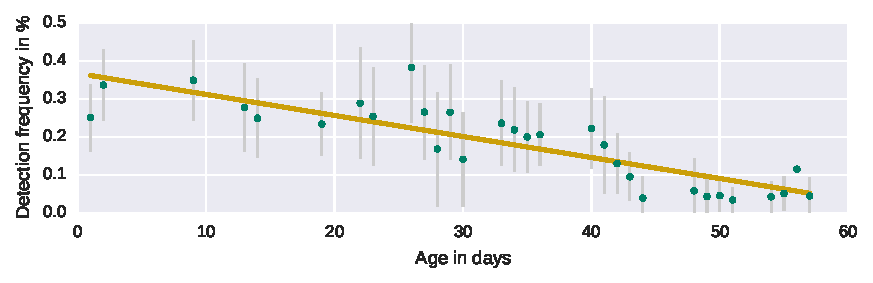
\includegraphics[width=1.0\textwidth]{Figures/n3_detFvsAge}
	\caption[Correlation]{Correlation of detection frequency and age}
	\label{fig:n3detfVSage}
	\end{subfigure} 
	\begin{subfigure}[b]{1\textwidth}
	\centering
	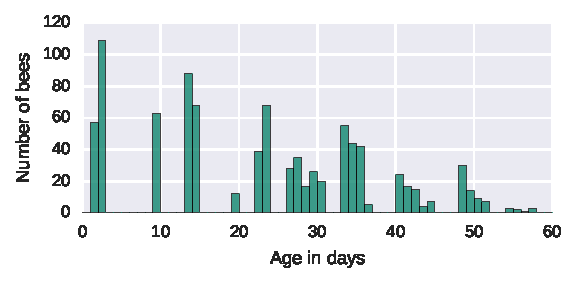
\includegraphics[width=1.0\textwidth]{Figures/n3_ages.pdf}
	\caption[Age distribution]{Age distribution}
	\label{fig:n3ageDist}
	\end{subfigure}
	\begin{subfigure}[b]{1\textwidth}
	\centering
	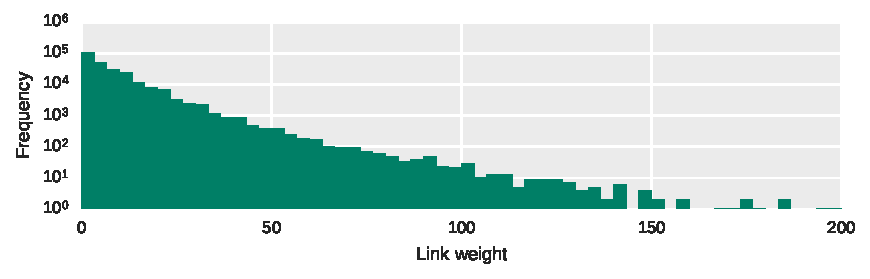
\includegraphics[width=1.0\textwidth]{Figures/n3-edgeWeightDist.pdf}
	\caption[Edge weight distribution]{Edge weight distribution}
	\label{fig:edgeWdist}
	\end{subfigure}
	\caption[Age distribution, correlation with detection frequency and edge weight distribution of snapshot~3]{\textbf{Age distribution, correlation with detection frequency and edge weight distribution of snapshot~3} (a) Detection frequency and the age of a honeybee seem to be negatively correlated. (b) The age of bees ranges from $1$ to $60$ days, but some age groups are missing. (c) The edge weight distribution decays exponentially.}
	\label{fig:ageDetF}
\end{figure}